\chapter{Classifier}

k-nearest neighborhood

one of the simplest

Tree, random forest

Decision tree: can be used for classification or regression
It can be represented as a graph and a simple representation is given \ref{fig:decision_tree_simple_example}.

\begin{figure}[h]
    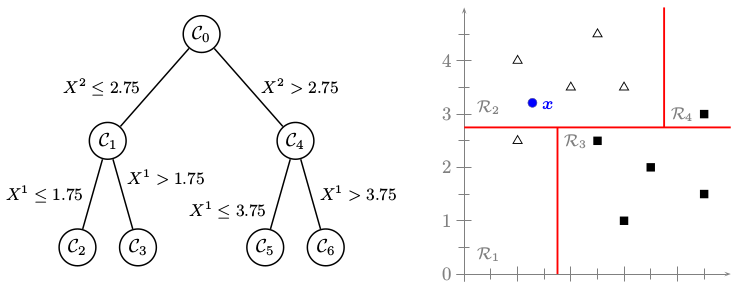
\includegraphics[scale=0.5]{img/decision_tree_simple_example}
    \caption{Decision tree of depth 2 for 10 elements belonging to 2 classes}
    \label{fig:decision_tree_simple_example}
\end{figure}


Naive bayesian

SVM (binary case) + kernel trick + multi-class (one-versus-one or one-versus-all)

The Support Vector Machine (SVM) is a method used for classification and regression. A support vector machine constructs a hyper-plane or set of hyper-planes in a high or infinite dimensional space, which can be used for classification, regression or other tasks. Intuitively, a good separation is achieved by the hyper-plane that has the largest distance to the nearest training data points of any class (so-called functional margin), since in general the larger the margin the lower the generalization error of the classifier.

To generalize SVM to the case of multi-class, multiple approaches are possible:
\begin{itemize}
    \item \enquote{one-versus-one}: train a separate classifier for each different pair of labels. This leads to $\frac{N (N - 1)}{2}$ classifiers
    \item \enquote{one-versus-all}: train a single classifier per class, with the samples of that class as positive samples and all other samples as negatives
\end{itemize}

Kernel trick:
to use the linear SVM for non-linear data: project the data in a new feature H space thanks to an application and then reserch for maximum margin hyperplan in H
to make sure that the new problem has a unique solution, 
must satisfy the Mercer's condition or simply it must be a positiv-definit matrix

\begin{itemize}
    \item \textbf{Linear} : $k(x, y) = \langle \vec{x} , \vec{y} \rangle + C = x^T y + C$
    \item \textbf{Polynomial}: $k(x, y) = (\gamma \cdot \langle \vec{x} , \vec{y} \rangle + C)^d = (\gamma \times x^T y + C)^d$
    \item \textbf{Radial Basis Function (RBF)}: $k(x, y) = \exp \left( - \gamma \lVert x - y \rVert ^2 \right)$
    \item \textbf{Chi-Square}: $\displaystyle k(x, y) = 1 - \sum_{i=1}^n \frac{(x_i-y_i)^2}{\frac{1}{2} (x_i+y_i)}$
    
    A modified version presented in \cite{Vedaldi2010} of this kernel is the \textbf{Additive Chi-Square} kernel :
    $\displaystyle k(x, y) = \sum_{i=1}^n \frac{2 (x_i - y_i)}{x_i + y_i} $
\end{itemize}

The adjustable parameters of these kernels are $d$, $\gamma$, $C$ and must be choosen according to the problem.

SGD classifier + loss function + regularization term% http://scikit-learn.org/stable/modules/sgd.html#mathematical-formulation

CNN

inspired by the neural system composed of different layers and communication shemes
recent years: use of the adjectiv "deep" to qualify NN: many layers

Different types of layers:
% http://cs231n.github.io/convolutional-networks/
% http://caffe.berkeleyvision.org/tutorial/layers.html
% Vision
- convolutional (give the name of the type of NN) : The Convolution layer convolves the input image with a set of learnable filters, each producing one feature map in the output image.
- max pooling
- normalization layer % http://stats.stackexchange.com/a/161200
% Loss layer
- sigmoid
% Activation / Neuron Layers
- ReLu